%&pdflatex
\documentclass[mathserif]{beamer} %, handout
\usetheme[progressbar=foot]{metropolis}
\setbeamertemplate{caption*}[numbered]

\usepackage[utf8x]{inputenc}
\usepackage[T2A]{fontenc}
\usepackage[english,russian]{babel}

\usepackage{amssymb, amsmath, amsfonts, mathtools, mathrsfs}
\usepackage[normalem]{ulem} % for sout
\usepackage{comment}
\usepackage{changepage} % for adjustwidth
\usepackage{tabu, tabulary}
\usepackage{extarrows} % for xlongequal

\usepackage{subcaption}
\usepackage{tikz}
\usepackage{pgfplots}
\usetikzlibrary{arrows.meta}

\title{Некоторые вопросы функционального, асимптотического и численного анализа больцмановской динамики}
\author{Рогозин Олег Анатольевич}
\institute{
    Вычислительный центр ФИЦ ИУ РАН
}
\date{}

\newcommand{\Kn}{\mathrm{Kn}}
\newcommand{\St}{\mathrm{St}}
\newcommand{\Ma}{\mathrm{Ma}}
\newcommand{\loc}{\mathrm{loc}}
\newcommand{\eqdef}{\mathrel{\overset{\makebox[0pt]{\mbox{\normalfont\tiny\sffamily def}}}{=}}}
\newcommand{\dd}{d}%{\:\mathrm{d}}
\newcommand{\pder}[2][]{\frac{\partial#1}{\partial#2}}
\newcommand{\pderdual}[2][]{\frac{\partial^2#1}{\partial#2^2}}
\newcommand{\pderder}[3][]{\frac{\partial^2#1}{\partial#2\partial#3}}
\newcommand{\Pder}[2][]{\partial#1/\partial#2}
\newcommand{\der}[2][]{\frac{\dd#1}{\dd#2}}
\newcommand{\derdual}[2][]{\frac{\dd^2#1}{\dd#2^2}}
\newcommand{\Der}[2][]{\dd#1/\dd#2}
\newcommand{\dxi}{\boldsymbol{\dd\xi}}
\newcommand{\bxi}{\boldsymbol{\xi}}
\newcommand{\bh}{\boldsymbol{h}}
\newcommand{\be}{\boldsymbol{e}}
\newcommand{\bv}{\boldsymbol{v}}
\newcommand{\bx}{\boldsymbol{x}}
\newcommand{\OO}[1]{O(#1)}
\newcommand{\Nu}{\mathcal{N}}
\newcommand{\Mu}{\mathcal{M}}
\newcommand{\Set}[2]{\{\,{#1}:{#2}\,\}}
\newcommand{\xoverbrace}[2][\vphantom{\int}]{\overbrace{#1#2}}
\newcommand{\Cite}[2][]{\alert{\textsc{#2 #1}}}
\newcommand{\inner}[2]{\left\langle{#1},{#2}\right\rangle}
\newcommand{\onwall}[1]{\left(#1\right)_0}
\newcommand{\deltann}[2]{(\delta_{#1#2}-n_#1 n_#2)}

\newcommand\pro{\item[$+$]}
\newcommand\con{\item[$-$]}

% use Russian tradition
\renewcommand{\phi}{\varphi}
\renewcommand{\epsilon}{\varepsilon}

\begin{document}

\frame{\titlepage}

\begin{frame}
    \frametitle{Содержание}
    \linespread{0.8}
    \tableofcontents
\end{frame}

\section{Кинетическая теория}

\begin{frame}
    \frametitle{Функция распределения молекулярных скоростей}
    Микроскопическое описание (гамильтониан):
    \begin{equation*}
        H(\bx,\bxi) = \frac12 \sum_{i=1}^{N}|\bxi_i|^2 + \sum_{i\ne j} U(\bx_i - \bx_j).
    \end{equation*}
    Мезоскопическое описание (функция распределения): % минимальные предположения
    \begin{equation*}
        f(t,\bx,\bxi): \mathbb{R}_+\times\Omega\times\mathbb{R}^d\mapsto\mathbb{R}_+
        \quad (\Omega\subset\mathbb{R}^d),
    \end{equation*}
    \begin{equation*}
        f(t,\cdot,\cdot) \in L^1_\loc(\Omega; L^1(\mathbb{R}^d)).
    \end{equation*}
    Макроскопическое описание (поля): % часто более гладкие, чем ФР
    \begin{gather*}
        \rho = \int_{\mathbb{R}^d} f\dxi, \\
        \bv = \frac1\rho\int_{\mathbb{R}^d} \bxi f\dxi, \\
        T = \frac1{d\rho}\int_{\mathbb{R}^d} \left(|\bxi|^2 - |\bv|^2\right) f\dxi.
    \end{gather*}
\end{frame}

\begin{frame}
    \frametitle{Уравнение Больцмана}
    \Cite[1872]{Boltzmann}:
    \begin{equation*}
        \pder[f]{t} + \xi_i\pder[f]{x_i} = J(f,f).
    \end{equation*}

    \begin{itemize} % с точки зрения энтропии
        \item \(\xi_i\pder{x_i}\) "--- транспортный оператор (консервативный)
        \item \(J(f,f)\) "--- столкновительный оператор (диссипативный)
    \end{itemize}

    \begin{gather*}
        J(f,f)(t,\bx,\bxi) \eqdef \int_{\mathbb{R}^d}\dxi_* \int_{S^{d-1}} \boldsymbol{\dd\alpha}
        \overbrace{B(\bxi-\bxi_*,\boldsymbol\alpha)}^\text{collisional kernel}
        \Big( \overbrace{f'f'_*}^\text{gain} - \overbrace{ff_*}^\text{loss} \Big), \\
        f=f(\xi), \quad f_*=f(\xi_*), \quad f'=f'(\xi), \quad f'_*=f(\xi'_*).
    \end{gather*}
    Скорости после столкновения:
    \begin{equation*}
        \xi_i' = \xi_i+\alpha_i\alpha_j (\xi_{j*}-\xi_j), \quad \xi_{i*}' = \xi_{i*}-\alpha_i\alpha_j (\xi_{j*}-\xi_j).
    \end{equation*}
\end{frame}

\begin{frame}
    \frametitle{Симметрии и H-теорема Больцмана}
    Слабая формулировка:
    \begin{equation*}
        \int_{\mathbb{R}^d} J(f,f)\alert{\phi}\dxi = \frac14 \int_{\mathbb{R}^d} J(f,f) (\phi + \phi_* - \phi' - \phi'_*)\dxi.
    \end{equation*}
    \pause
    Законы сохранения:
    \begin{equation*}
        \int_{\mathbb{R}^d} J(f,f)\alert{\begin{pmatrix}
            1 \\ \xi_i \\ \xi^2
        \end{pmatrix}}\dxi = 0.
    \end{equation*}
    \pause
    Функционал производства энтропии:
    \begin{equation*}
        \mathcal{D}(f) \eqdef -\int_{\mathbb{R}^d} J\alert{\log{f}} = \frac14\int_{\mathbb{R}^{2d}\times S^{d-1}}
        B\left( f'f'_* - ff_* \right) \log\frac{f'f'_*}{ff_*} \geq 0.
    \end{equation*}
    Функционал Ляпунова / \(\mathcal{H}\)-функционал / отриц. энтропия:
    \begin{equation*}
        \mathcal{H}(f) \eqdef \int_{\Omega\times\mathbb{R}^d} f\log{f} \xrightarrow{t\to\infty} \min,
        \quad \der[\mathcal{H}]{t} \xlongequal{\mathcal{H}\text{-теорема}} - \int_\Omega D \leq 0.
    \end{equation*}
\end{frame}

\begin{frame}
    \frametitle{Классификация столкновительных ядер}
    \begin{gather*}
        U(r)\sim r^{1-s} \:\implies\: \sin^{d-1}\theta B(|\bxi-\bxi_*|,\cos\theta)
            \overset{d=3}{\sim} |\bxi-\bxi_*|^\gamma \theta^{-1-\nu}, \\
        \quad \gamma = \dfrac{s-5}{s-1}\in[-3,1), \quad \nu = \dfrac2{s-1}\in(0,2], \\
        \int_0^\pi \theta^{-1-\nu}\dd\theta = +\infty\:\implies\:\int_{S^2} B\boldsymbol{\dd\alpha} = +\infty,
            \quad \theta\text{ --- угол разлёта.}
    \end{gather*}
    \vspace{-10pt}
    \begin{itemize}
        \item твёрдые сферы: \(s=+\infty,\:\gamma=1,\:\nu=0 \:\implies\:\) \framebox{\(B=|\bxi-\bxi_*|\)}
        \item жёсткие потенциалы: \(\gamma>0\)
        \item максвелловские молекулы: \(s=5,\:\gamma=0,\:\nu=\frac12\)
        \item мягкие потенциалы: \(\gamma<0\)
        \item кулоновский: \(s=2,\:\gamma=-3,\:\nu=2\) \(\:\longrightarrow\:\) уравнение Ландау,\\
            \Cite[1936]{Landau}, \Cite[1990]{Arsen'ev, Buryak} \\
            {\footnotesize Арсеньев Алексей Алексеевич (1938--2013, МГУ)}
    \end{itemize}
\end{frame}

\begin{frame}
    \frametitle{Кинетические граничные условия}
    \vspace{-10pt}
    \begin{equation*}
        f_B(\bx,\bxi) = \int_{\xi_{*i}n_i<0} \overbrace{\mathcal{R}(\bxi,\bxi_*,\bx)}^\text{scattering kernel}f(\bx,\bxi_*)\dxi_*
        \quad \left( x\in\partial\Omega,\:\xi_in_i>0 \right),
    \end{equation*}
    \vspace{-10pt}
    \begin{itemize}
        \item \(n_i\) "--- единичная нормаль, направленная в сторону газа,
    \end{itemize}
    \begin{gather*}
        \mathcal{R}(\bxi,\bxi_*) \geq 0, \\ % положительность
        -\int_{\xi_in_i>0} \frac{\xi_kn_k}{\xi_{j*}n_j}
            \mathcal{R}(\bxi,\bxi_*)\dxi = 1, \\ % непористой и неабсорбирующей
        \int_{\xi_{*i}n_i<0} \mathcal{R}(\bxi,\bxi_*)f_B(\bxi_*)\dxi_* = f_B(\bxi),
            \quad f_B = f_M(\rho_B, \bv_B, T_B). % для ядра, зависящего от плотности, скорости и температуры границы
    \end{gather*}
    Однопараметрическая модель Максвелла:
    \begin{equation*}
            \mathcal{R}_\mathrm{M} = \alert{(1-\alpha_\mathrm{M})}\delta\left( \xi_{i*} - \xi_i + 2\xi_jn_jn_i \right)
            -\frac{2\alert{\alpha_\mathrm{M}}}{\pi T_B^2} \xi_{j*}n_j \exp\left( -\frac{(\xi_k-v_{Bk})^2}{T_B} \right).
    \end{equation*}
\end{frame}

\section{Асимптотическая теория}

\begin{frame}
    \frametitle{Формальная асимптотическая теория для \(\Ma = \OO{1}\)}
    \[ \St \pder[f]{t} + \xi_i\cdot\pder[f]{x_i} = \frac1{\Kn} J(f,f) \]
    Гидродинамический предел: \(\Kn\to0\), классификация по \(\St\):
    \begin{itemize}
        \item начальный слой \(\St = \OO{\Kn^{-1}}\)
        \item акустический (невязкий) режим \(\St = \OO{1}\)
        \item диффузионный (вязкий) режим \(\St = \OO{\Kn}\)
    \end{itemize}
    \begin{itemize}
        \item \Cite[1912]{Hilbert}: \( f = \sum_{n=0}^\infty \Kn^n f_n(\bx,\bxi,t) \)
        \item \Cite[1917]{Enskog}: \( f = \sum_{n=0}^\infty \Kn^n f_n(\rho_r,\nabla\rho_r,\bxi) \)
        \item \Cite[1982]{Bobylev}: акустическая нестабильность уравнений Барнетта
        % амплитуда акустических волн, описываемых уравнениями Барнетта для максвелловских молекул, растёт со временем
    \end{itemize}
\end{frame}

\begin{frame}
    \frametitle{Формальная асимптотическая теория для \(\Ma = \OO{1}\)}
   	\begin{columns}
		\column{.55\textwidth}
		\begin{center}
		    \vspace{-27pt}
            \footnotesize
            \begin{tikzpicture}[arrow/.style={>={Stealth[scale length=1.5]}, thin, shorten <=.3pt}]
                \pgftransformscale{3}
                \clip (-0.5,2) rectangle (1.5,5);
                \fill[fill=black!20, draw=black, very thick] (0,0) circle [radius=2.5];
                \foreach \i in {.65,1,2}
                    \draw[semithick] (0,0) circle [radius=2+\i];
                \node at (0,2.58) {Соне};
                \node at (0,2.83) {Кнудсен};
                \node at (0,3.5) {Прандтль};
                \node at (0,4.5) {Эйлер};
                \draw[<->, arrow] (81:2.5) -- (81:4) node [right,midway] {\(\OO{\sqrt{k}}\)};
                \draw[<->, arrow] (73:2.5) -- (73:3) node [right,midway] {\(\OO{k}\)};
                \draw[thin] (65:2.3) node [above left=-2pt] {\(\OO{k^2}\!\)}  -- (65:2.85);
                \draw[>-<, arrow, shorten <=-7pt, shorten >=-7pt] (65:2.5) -- (65:2.65) ;
            \end{tikzpicture}
        \end{center}
		\column{.5\textwidth}
		\vspace{-10pt}
		\begin{itemize}
			\item область невязкого течения: \[ \pder[f]{x_i}n_i = \OO{f} \]
			\item вязкостный слой (Прандтля):\!\!\!\!\!\!\!\!\! \[ \sqrt{\Kn}\pder[f]{x_i}n_i = \OO{f} \]
			\item слой Кнудсена: \[ \Kn\pder[f]{x_i}n_i = \OO{f} \]
			\item слой Соне (\Cite[1973]{Sone}): \[ \pder[f]{x_i}n_i \to \infty \]
		\end{itemize}
	\end{columns}
\end{frame}

\begin{frame}
    \frametitle{Разложение Гильберта для медленных течений}
    Стационарное уравнение Больцмана в присутствии внешней силы
    \begin{equation}\label{eq:Boltzmann}
        \xi_i\pder[f]{x_i} + F_i\pder[f]{\xi_i} = \frac1k J(f,f).
    \end{equation}
    Разложение по числу Кнудсена \(k=\Kn\sqrt\pi/2\):
    \begin{equation}\label{eq:expansion}
        f = f_0 + f_1k + f_2k^2 + \cdots, \quad h = h_0 + h_1k + h_2k^2 + \cdots,
    \end{equation}
    где макроскопические величины \(h = \rho, v_i, T, \dots\)
    \vspace{5pt}\pause

    Предположения:
    \begin{itemize}
        \item медленные течения \(\int\xi_i f\dxi = v_i = \OO{k}\) (\(\mathrm{Re} = \OO{1}\))
        \item слабая внешняя сила \(F_i = \OO{k^2}\)
    \end{itemize}
    Из-за вырожденности уравнения движения
    \begin{equation}
        \pder[p_0]{x_i} = 0, \quad \pder[p_1]{x_i} = 0.
    \end{equation}
\end{frame}

\begin{frame}
    \frametitle{Уравнения гидродинамического типа}
    \Cite[1970, 1971, 1976]{Коган, Галкин, Фридлендер}:
    \begin{align*}
        \pder{x_i}\left(\frac{u_{i1}}{T_0}\right) &= 0, \\
        \pder{x_j}\left(\frac{u_{i1}u_{j1}}{T_0}\right)
            &-\frac12\pder{x_j}\left[\Gamma_1\left(
                \pder[u_{i1}]{x_j} + \pder[u_{j1}]{x_i} - \frac23\pder[u_{k1}]{x_k}\delta_{ij}
            \right)\right] \notag\\
            &-\alert{\left[
                \frac{\Gamma_7}{\Gamma_2}\frac{u_{j1}}{T_0}\pder[T_0]{x_j}
                + \frac{\Gamma_2^2}4 \left(\frac{\Gamma_7}{\Gamma_2^2}\right)'
                    \left(\pder[T_0]{x_j}\right)^2
            \right]\pder[T_0]{x_i}} \notag\\
            &= -\frac12\pder[p_2^\dag]{x_i} + \frac{p_{H0}^2 F_{i2}}{T_{0}}, \\
        \pder[u_{i1}]{x_i} &= \frac12\pder{x_i}\left(\Gamma_2\pder[T_0]{x_i}\right),
    \end{align*}
    где
    \begin{equation*}
        p_2^\dag = p_0 p_2
            + \frac23\pder{x_k}\left(\alert{\Gamma_3}\pder[T_0]{x_k}\right)
            - \frac{\alert{\Gamma_7}}{6}\left(\pder[T_0]{x_k}\right)^2, \quad u_{i1} = p_0v_{i1}.
    \end{equation*}
\end{frame}

\begin{frame}
    \frametitle{Уравнения гидродинамического типа}
    \centering{\Large\bf Как их назвать?}
    \vspace{10pt}
    \begin{itemize}
        \item SNF/SNIF equations \Cite[1993]{Kogan}, \Cite[1995]{Bobylev}
        \item ghost effect equations \Cite[2009]{Levermore+}, \Cite[2017]{Aoki+}
        \item уравнения Когана"--~Галкина"--~Фридлендера \Cite[2017]{Рогозин}
    \end{itemize}
    \vspace{20pt}
    \centering{\Large\bf Экспериментальное подтверждение}
    \begin{itemize}
        \item \Cite[1997, 2003]{Friedlander, Nikolsky et al.}:\\
            в вакуумной аэродинамической трубе ЦАГИ (ВАТ-2М)
    \end{itemize}
\end{frame}

\begin{frame}
    \frametitle{Действующие силы}
    На единицу массы газа действует сила
    \begin{equation}\label{eq:gamma7_force}
        F_i = -\frac{\alert{\Gamma_7(T)}}{4p_H} \left(\pder[T_H]{x_j}\right)^2 \pder[T_H]{x_i} k^2 + \OO{k^3},
    \end{equation}
    Она вызывает \alert{нелинейное термострессовое течение}.\\
    Для степенного потенциала
    \[ \Gamma_{1,2}(T) = \gamma_{1,2}T^s, \quad \Gamma_3(T) = \gamma_3T^{2s},
        \quad \alert{\Gamma_7(T)} = \Gamma_3' - \gamma_7T^{2s-1}. \]
    \pause\vspace{-10pt}

    Сила, действующая на равномерно нагретое покоящееся тело,
    \begin{multline}\label{eq:force:terms}
        p_0 \oint_S F_{i2} \dd{S} =
            - \overbrace{ \oint_S p_2^\dag n_i \dd{S} }^\text{pressure} \\
            + \underbrace{ \Gamma_1\oint_S \pder[u_{i1}]{x_j} n_j \dd{S} }_\text{viscosity}
            + \underbrace{ \frac{\Gamma_7}{2} \oint_S \left(\pder[T_0]{x_j}\right)^2 n_i \dd{S} }_\text{thermal-stress}.
    \end{multline}
\end{frame}

\begin{frame}
    \frametitle{Слой Кнудсена первого порядка}
    \begin{equation}
        \alert{T_0} = T_{B0}. \label{eq:bc_T0}
    \end{equation}

    \begin{gather}
        \frac{p_0}{T_{B0}}
            \begin{bmatrix} \alert{T_1} - T_{B1} \\ T_{K1} \\ T_{B0}^2\rho_{K1} \end{bmatrix} =
            \onwall{\pder[T_0]{x_j}} n_j \begin{bmatrix} d_1 \\ \Theta_1(\eta) \\ p_0\Omega_1(\eta) \end{bmatrix}, \\
        \left\{
        \begin{aligned}
            & \frac1{\sqrt{T_{B0}}}\begin{bmatrix} (\alert{u_{j1}} - u_{Bj1}) \\ u_{jK1} \end{bmatrix} \deltann{i}{j} =
                \onwall{\pder[T_0]{x_j}}\begin{bmatrix} k_0 \\ Y_0(\eta) \end{bmatrix}\deltann{i}{j}, \\
            & \alert{u_{j1}} n_j = 0.
        \end{aligned}
        \right.
    \end{gather}
    \vspace{-20pt}
    \begin{itemize}
        \item \(\eta = \frac{p_0}{T_{B0}}(x_i-x_{Bi})\frac{n_i}k \) "--- растянутая нормальная координата
        \item \(\Theta_1, \Omega_1, Y_0 = \OO{\eta^{-\infty}}\)
        \item \(\onwall{\cdots}\) "--- значение на границе (\(\eta=0\))
    \end{itemize}
\end{frame}

\begin{frame}
    \frametitle{Слой Кнудсена второго порядка}
    \footnotesize
    \begin{equation*}
        \begin{aligned}
            \frac1{\sqrt{T_{B0}}}&
                \begin{bmatrix} (u_{j2} - u_{Bj2}) \\ u_{jK2} \end{bmatrix}\deltann{i}{j} = \\
            &- \left.\frac{\sqrt{T_{B0}}}{p_0}\onwall{\pder[u_{j1}]{x_k}} \deltann{i}{j}n_k
                \begin{bmatrix} k_0 \\ Y_0(\eta) \end{bmatrix} \quad\right\}\text{velocity jump}\\
            &- \left.\frac{T_{B0}}{p_0}\onwall{\pderder[T_0]{x_j}{x_k}} \deltann{i}{j}n_k
                \begin{bmatrix} a_4 \\ Y_{a4}(\eta) \end{bmatrix} \quad\right\}\text{thermal slip} \\
            &\left.\begin{aligned}
                &- \bar\kappa\frac{T_{B0}}{p_0}\onwall{\pder[T_0]{x_j}} \deltann{i}{j}
                \begin{bmatrix} a_5 \\ Y_{a5}(\eta) \end{bmatrix} \\
                &- \kappa_{jk}\frac{T_{B0}}{p_0}\onwall{\pder[T_0]{x_k}} \deltann{i}{j}
                \begin{bmatrix} a_6 \\ Y_{a6}(\eta) \end{bmatrix}
            \end{aligned} \quad\right\}\text{curvature terms}\\
            &- \left.\pder[T_{B1}]{x_j} \deltann{i}{j}
                \begin{bmatrix} K_1 \\ \frac12 Y_1(\eta) \end{bmatrix}. \quad\right\}\text{thermal creep}
        \end{aligned}\label{eq:boundary_u2t}
    \end{equation*}
    \vspace{-10pt}
    \begin{itemize}
        \item \(\kappa_{ij} = \kappa_1 l_i l_j + \kappa_2 m_i m_j\) "--- тензор кривизны, \(\bar\kappa = (\kappa_1+\kappa_2)/2\)
    \end{itemize}
\end{frame}

\begin{frame}
    \frametitle{Слой Кнудсена второго порядка}
    \footnotesize
    \begin{gather*}
        \begin{multlined}
            \frac1{\sqrt{T_{B0}}}
                \begin{bmatrix} (u_{j2} - u_{Bj2}) \\ u_{jK2} \end{bmatrix} n_j = \\
            - \frac{T_{B0}}{p_0}\left[ \onwall{\pderder[T_0]{x_i}{x_j}}n_i n_j
                + 2\bar\kappa\onwall{\pder[T_0]{x_i}}n_i \right]
                \begin{bmatrix} \frac12\int_0^\infty Y_1(\eta_0)\dd\eta_0 \\
                    \frac12\int_\infty^{\eta} Y_1(\eta_0)\dd\eta_0 \end{bmatrix}.
        \end{multlined}\label{eq:boundary_u2n}\\
        \begin{aligned}
            \frac{p_0}{T_{B0}}
                \begin{bmatrix} T_2 - T_{B2} \\ T_{K2} \\ T_{B0}^2\rho_{K2} \end{bmatrix}
            &= \onwall{\pder[T_1]{x_j}} n_j
                \begin{bmatrix} d_1 \\ \Theta_1(\eta) \\ p_0\Omega_1(\eta) \end{bmatrix} \\
            &+ \frac{T_{B0}}{p_0}\onwall{\pderder[T_0]{x_i}{x_j}} n_i n_j
                \begin{bmatrix} d_3 \\ \Theta_3(\eta) \\ p_0\Omega_3(\eta) \end{bmatrix} \\
            &+ \bar\kappa\frac{T_{B0}}{p_0}\onwall{\pder[T_0]{x_i}} n_i
                \begin{bmatrix} d_5 \\ \Theta_5(\eta) \\ p_0\Omega_5(\eta) \end{bmatrix}.
        \end{aligned}\label{eq:boundary_T2}
    \end{gather*}
\end{frame}

\section{Течение между некоаксиальными цилиндрами}

\begin{frame}
    \frametitle{Поле скоростей в континуальном пределе}
    \centering
    \begin{figure}
    \begin{overprint}
        \onslide<1| handout:2>
            \[ T_1 = 1, \quad T_2 = 5.\]
            \hspace{-1cm}
            \includegraphics[width=1.15\linewidth]{noncoaxial/cylinder5}
        \onslide<2| handout:1>
            \[ T_1 = 5, \quad T_2 = 1.\]
            \hspace{-1cm}
            \includegraphics[width=1.15\linewidth]{noncoaxial/inverse5}
        \onslide<3| handout:0>
            \[ T_1 = 1, \quad T_2 = 50.\]
            \hspace{-1cm}
            \includegraphics[width=1.15\linewidth]{noncoaxial/cylinder50}
    \end{overprint}
    \hspace{-.5cm}
    \end{figure}
\end{frame}

\begin{frame}
    \frametitle{Зависимость поля скоростей от \(\tau = T_2-T_1\)}
    \centering
    \begin{columns}
        \column{.7\textwidth}
        \begin{figure}
            \includegraphics[width=\linewidth]{noncoaxial/U-tau-cylinders}
            \vspace{-.5cm}\caption{максимальное значение скорости}
        \end{figure}
        \column{.4\textwidth}
        \[ u_{i1} = \OO{\tau^3}, \quad \tau\to0, \]
        \[ u_{i1} = \OO{\tau^{3/2}}, \quad \tau\to\infty. \]
    \end{columns}
\end{frame}

\begin{frame}
    \frametitle{Зависимость действующей силы от \(\tau = T_2-T_1\)}
    \vspace{-.2cm}
    \[ p_0 \oint_S F_{x2}\dd{S} = \OO{\tau^2}. \]
    \vspace{-.7cm}
    \begin{columns}
        \column{.6\textwidth}
        \begin{figure}
            \includegraphics[width=\linewidth]{noncoaxial/F-tau-cylinders-inner}
            \vspace{-.5cm}\caption{внутренний цилиндр}
        \end{figure}
        \column{.6\textwidth}
        \begin{figure}
            \includegraphics[width=\linewidth]{noncoaxial/F-tau-cylinders-outer}
            \vspace{-.5cm}\caption{внешний цилиндр}
        \end{figure}
    \end{columns}
\end{frame}

\begin{frame}
    \frametitle{Зависимость действующей силы от расстояния между осями}
    \vspace{-.5cm}
    \[ p_0 \oint_S F_{x2}\dd{S} = \begin{cases}
        \OO{(1-d)^{-1}} & \quad\text{для cфер}, \\
        \OO{(1-d)^{-3/2}} & \quad\text{для цилиндров}, \\
        \end{cases} \quad d\to1. \]
    \vspace{-.7cm}
    \begin{columns}
        \column{.6\textwidth}
        \begin{figure}
            \includegraphics[width=\linewidth]{noncoaxial/forces}
        \end{figure}
        \column{.6\textwidth}
        \begin{figure}
            \includegraphics[width=\linewidth]{noncoaxial/forces-close}
        \end{figure}
    \end{columns}
\end{frame}

\begin{frame}
    \frametitle{Электростатическая аналогия}
    \footnotesize
    Транспортные коэффициенты для степенных потенциалов:
    \begin{equation*}\label{eq:gammas}
        \Gamma_2 = \gamma_2 T^s, \quad \Gamma_7 = \gamma_7 T^{2s-1}.
    \end{equation*}
    Тогда при \(\int p_2^\dag\dd{V} = 0\)
    \begin{gather*}
        e_a \eqdef T_a^s \oint_{S_a} \pder[T_0]{x_i}n_i\dd{S} = C_{ab} T_b^{1+s}, \quad \sum_a e_a = 0, \\
        U \eqdef \int \left[ \frac{\Gamma_7}2\left(\pder[T_0]{x_i}\right)^2 - p_2^\dag \right]\dd{V} =
        \gamma_7 \sum_a T_a^{2s} \oint_{S_a} \pder[T_0]{x_i}n_i\dd{S} = C_{ab} T_a^s T_b^{1+s}, \\
        F^a_i \eqdef \oint_{S_a} \left( \frac{\Gamma_7}{2}\left(\pder[T_0]{x_j}\right)^2 - p_2^\dag \right) n_i\dd{S}
            = \frac{\delta C_{ab}}{\delta x_i} T_a^s T_b^{1+s}.
    \end{gather*}
    Для двух тел
    \begin{equation*}
        F_i \propto \left( T_2^s - T_1^s \right)\left( T_2^{1+s} - T_1^{1+s} \right) \quad (s\neq0,-1).
    \end{equation*}
    Для цилиндров и сфер:
    \begin{equation*}
        C_\mathrm{cyl} \propto \frac1{\theta}, \quad
        C_\mathrm{sph} \propto  \sum_{n=1}^\infty \frac{R_1 R_2 \sinh\theta} {R_2\sinh n\theta - R_1\sinh (n-1)\theta},
        \quad \cosh\theta = \frac{R_1^2 + R_2^2 - d^2}{2 R_1 R_2}.
    \end{equation*}
\end{frame}

\begin{frame}
    \frametitle{Электростатическая аналогия}
    \centering
    Зависимость силы притяжения двух тел \(F\) от разности температур \(\tau=T_2-T_1\) при \(T_1=1\).
    \begin{figure}[ht]
        \footnotesize\centering
        \begin{subfigure}[b]{0.49\textwidth}
            \centering
            \hspace{-1.4cm}
            \begin{tikzpicture}
                \begin{loglogaxis}[width=1.2\linewidth,
                    xlabel=\(\tau\), ylabel=\(F\)]
                    \addplot gnuplot [raw gnuplot, mark=none, color=blue, thick]{
                        set logscale xy;
                        set xrange [1e-2:1e3];
                        plot ((x+1)**.5-1)*((x+1)**1.5-1);
                    };
                    \addplot gnuplot [raw gnuplot, mark=none, color=black, very thin, dashed]{
                        set xrange [1e0:1e3];
                        plot x**2;
                    };
                    \addplot gnuplot [raw gnuplot, mark=none, color=black, very thin, dashed]{
                        set xrange [1e-2:1e+2];
                        plot 3./4*x**2;
                    };
                \end{loglogaxis}
            \end{tikzpicture}
            \caption{газ твёрдых сфер (\(s=1/2\)).
                \(\frac34\tau^2\),~\(\tau\to0\) и \(\tau^2\),~\(\tau\to\infty\)}
        \end{subfigure}
        \begin{subfigure}[b]{0.49\textwidth}
            \centering
            \begin{tikzpicture}
                \begin{loglogaxis}[width=1.2\linewidth,
                    xlabel=\(\tau\), ylabel=\(F\)]
                    \addplot gnuplot [raw gnuplot, mark=none, color=blue, thick]{
                        set logscale xy;
                        set xrange [1e-2:1e3];
                        plot ((x+1)**1-1)*((x+1)**2-1);
                    };
                    \addplot gnuplot [raw gnuplot, mark=none, color=black, very thin, dashed]{
                        set samples 2;
                        set xrange [1e0:1e3];
                        plot x**3;
                    };
                    \addplot gnuplot [raw gnuplot, mark=none, color=black, very thin, dashed]{
                        set samples 2;
                        set xrange [1e-2:1e+1];
                        plot 2*x**2;
                    };
                \end{loglogaxis}
            \end{tikzpicture}
            \caption{максвелловский газ (\(s=1\)).
                \(2\tau^2\),~\(\tau\to0\) и \(\tau^3\),~\(\tau\to\infty\)}
        \end{subfigure}
    \end{figure}
\end{frame}

\section{Течение между эллиптическими цилиндрами}

\begin{frame}
    \frametitle{Поле скоростей в континуальном пределе}
    \[ T_1 = 1, \quad T_2 = 5.\]
    \centering
    \hspace{-1cm}
    \includegraphics[width=1.1\linewidth]{elliptic/U}
    \hspace{-1cm}
\end{frame}

\begin{frame}
    \frametitle{Момент действующей силы в континуальном пределе}
    \begin{columns}
        \column{.55\textwidth}
        \begin{figure}
            \includegraphics[width=\linewidth]{elliptic/moment-beta}
            \caption{полный момент сил}
        \end{figure}
        \column{.55\textwidth}
        \begin{figure}
            \includegraphics[width=\linewidth]{elliptic/profiles}
            \caption{профиль удельного момента}
        \end{figure}
    \end{columns}
\end{frame}

\begin{frame}
    \frametitle{Поле скоростей при \(\Kn=0.02\). \Cite[2017]{Rogozin}}
    \begin{figure}
        \hspace{-1cm}
        \begin{overprint}
            \onslide<1| handout:3>
                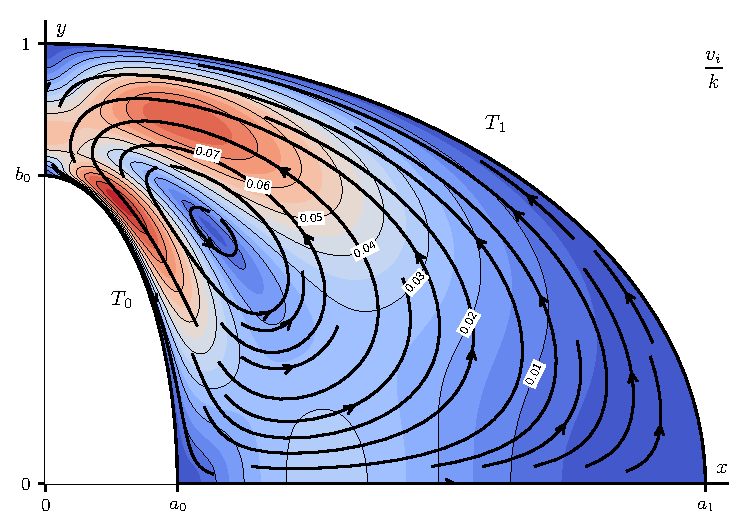
\includegraphics[width=\linewidth]{{{elliptic/kgf-0.02-flow}}}
                \vspace{-10pt}
                \caption{уравнения КГФ с граничными условиями ведущего порядка}
            \onslide<2| handout:2>
                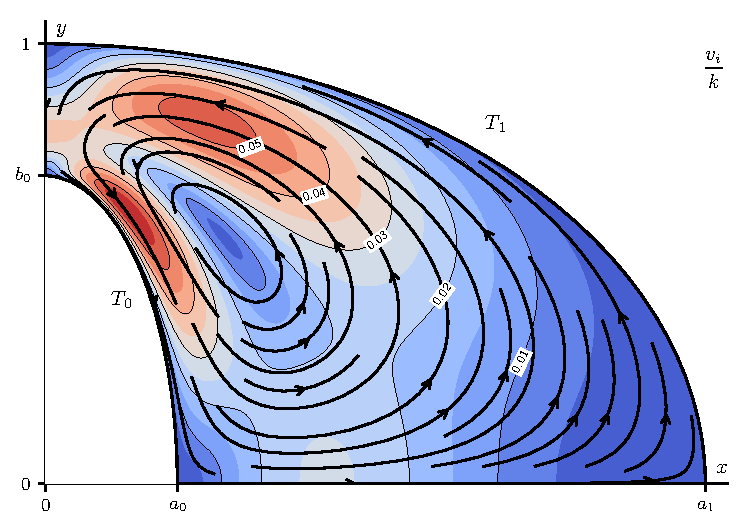
\includegraphics[width=\linewidth]{{{elliptic/first-0.02-flow}}}
                \vspace{-10pt}
                \caption{уравнения КГФ с граничными условиями первого порядка}
            \onslide<3| handout:1>
                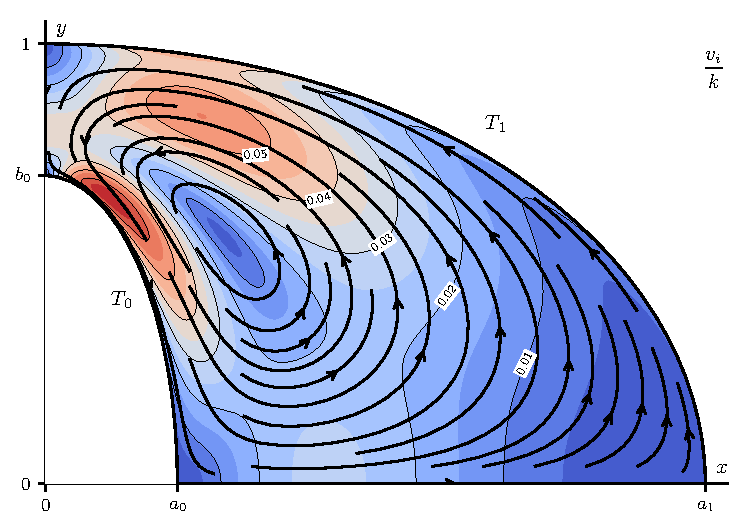
\includegraphics[width=\linewidth]{{{elliptic/second-0.02-flow}}}
                \vspace{-10pt}
                \caption{уравнения КГФ с граничными условиями второго порядка}
            \onslide<4| handout:0>
                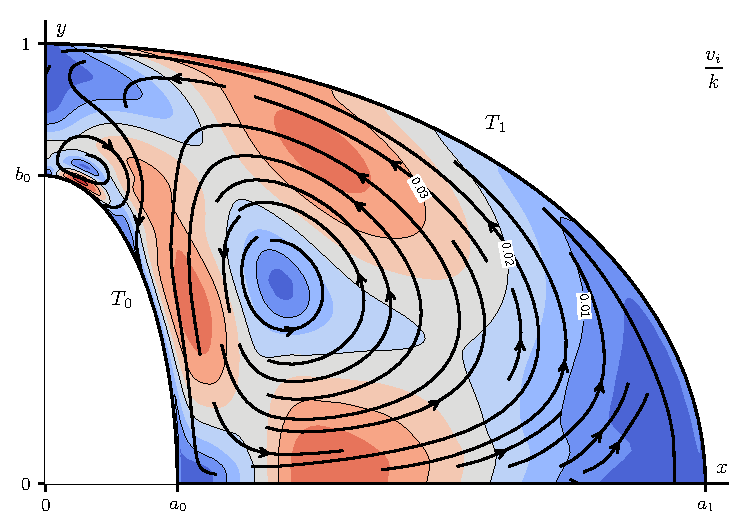
\includegraphics[width=\linewidth]{{{elliptic/kes-0.02-flow}}}
                \vspace{-10pt}
                \caption{численное решение уравнения Больцмана}
        \end{overprint}
    \end{figure}
\end{frame}

\section{Численные методы}

\begin{frame}
    \frametitle{Численные методы решения уравнения Больцмана}
    Ключевые свойства:
    \begin{itemize}
        \item сохранение массы, импульса и кинетической энергии;
        \item выполнение \(\mathcal{H}\)-теоремы;
        \item положительность \(f>0\).
    \end{itemize}
\end{frame}

\begin{frame}
    \frametitle{Классификация численных методов}
    \setlength{\leftmarginii}{10pt}
    \setlength{\leftmarginiii}{\leftmarginii}
    \begin{adjustwidth}{-2.5em}{-2.5em}
    \centering
    \newcommand{\ColW}{0.35\textwidth}
    \begin{tabular}{>{\centering\arraybackslash}p{\ColW}>{\centering\arraybackslash}p{\ColW}>{\centering\arraybackslash}p{\ColW}}
		\centering\bfseries Прямое статистическое моделирование &
		\centering\bfseries {Методы\\дискретных\\скоростей} &
		{\centering\bfseries Проекционные методы} \\
		\begin{itemize}
            \item метод Бёрда
            \begin{itemize}
                \pro неограниченное пространство скоростей
                \con сильный шум статистический
            \end{itemize}
            \item частицы с весом \(\rightarrow\) редкие события
            \item уменьшение дисперсии \(\rightarrow\) медленные течения
        \end{itemize} &
		\begin{itemize}
            \item прямое интегрирование
            \begin{itemize}
                \pro второй порядок
                \con неконсервативный
            \end{itemize}
            \item дискретный газ
            \begin{itemize}
                \pro консервативный
                \con дробный порядок
            \end{itemize}
            \item \alert{консервативное размазывание столкновительной сферы}
        \end{itemize} &
		\begin{itemize}
            \item Фурье--Галёркина (спектральный)
            \begin{itemize}
                \pro алгоритмы БПФ
                \pro спектральная точность
                \con неконсервативный
                \con явление Гиббса
            \end{itemize}
            \item разрывный Галёркин
            \begin{itemize}
                \pro высокий порядок точности
                \con осложнённый
            \end{itemize}
        \end{itemize} \\
	\end{tabular}
    \end{adjustwidth}
\end{frame}

\begin{frame}
    \frametitle{Консервативное размазывание столкновительной сферы}
    \centering
    {\Large Mетоды дискретных скоростей}\vspace{10pt}

    \Cite[1997]{Palczewski, Schneider, Bobylev}:\\
        сходимость дискретного газа < \(\frac14\) % Пальчевски, Шнайд'ер
    \vspace{10pt}
    \setlength{\leftmarginii}{10pt}
    \setlength{\leftmarginiii}{\leftmarginii}
    \begin{adjustwidth}{-2.5em}{-2.5em}
    \centering
    Computers \& Mathematics with Applications Vol. 35, No. 1-2\\
    (special issue edited by C.~Cercignani \& R.~Illner) % Рейнхард

    \newcommand{\ColW}{0.35\textwidth}
    \begin{tabular}{>{\centering\arraybackslash}p{\ColW}>{\centering\arraybackslash}p{\ColW}>{\centering\arraybackslash}p{\ColW}}
		\centering\bfseries Столкновительный интеграл &
		\centering\bfseries Столкновительная сфера &
		{\centering\bfseries Столкновительная пара} \\
		\Cite[1998]{Buet, Cordier, Degond} &
		\Cite[1998]{Babovsky}; \Cite[2002]{G\"orsch} &
		\Cite[1998]{Tcheremissine} \\
	\end{tabular}
    \end{adjustwidth}
\end{frame}

\begin{frame}
    \frametitle{Схема решения уравнения Больцмана}
    \vspace{-5pt}
    \[ \pder[f]{t} + \xi_i\pder[f]{x_i} = J(f,f) \]
    \vspace{-10pt}
    \begin{block}{Симметричная схема расщепления}
        \[ S_{A+B}^{\tau} = S_A^{\tau/2}S_B^{\tau}S_A^{\tau/2} + \OO{\tau^2} \]
        \centering \Cite[1968]{Strang}; \Cite[2001]{Bobylev, Ohwada}
    \end{block}
    \vspace{-10pt}
    \begin{columns}[T]
        \begin{column}{5cm}
            \begin{block}{Бесстолкновительное УБ}
                \[ \pder[f]{t} + \xi_i\pder[f]{x_i} = 0 \]
                \vspace{-15pt}
                \begin{itemize}
                    \item метод конечных объёмов
                    \item TVD-схема \(\OO{\tau^2, h^2}\)
                    \item (не)структурированная сетка
                \end{itemize}
            \end{block}
        \end{column}
        \begin{column}{6.5cm}
            \begin{block}{Пространственно-однородное УБ}
                \[ \pder[f]{t} = J(f,f) \]
                \vspace{-15pt}
                \begin{itemize}
                    \item проекционный метод дискретных скоростей
                    \item схема в дробных шагах \(\OO{\tau^2, h^2}\)
                    \item прямоугольная решётка
                \end{itemize}
            \end{block}
        \end{column}
    \end{columns}
\end{frame}

\begin{frame}
    \frametitle{Дискретизация пространства скоростей}
    % Группа для УБ, просто множество для модельных типа БГК
    Решётка \(\mathcal{V} = \Set{\xi_\gamma}{\gamma\in\Gamma}\) построена так, что
    \begin{equation}\label{eq:xi_cubature}
        \int F(\bxi) \dxi \approx \sum_{\gamma\in\Gamma} F_\gamma w_\gamma =
            \sum_{\gamma\in\Gamma} \hat{F_\gamma},
            \quad F_\gamma = F(\bxi_\gamma),
    \end{equation}
    \(\sum_{\gamma\in\Gamma} w_\gamma = V_\Gamma\) "--- объём, покрываемый скоростной решёткой.
    \pause\vspace{10pt}

    Симметризированный интеграл столкновений\vspace{-20pt}

    \begin{equation}\label{eq:symm_ci}
        J(f_\gamma, f_\gamma) = \frac14\int \left(
            \delta_\gamma + \delta_{\gamma*} - \delta'_\gamma - \delta'_{\gamma*}
        \right) (f'f'_* - ff_*)B \dd\Omega(\boldsymbol{\alpha}) \dxi\dxi_*
    \end{equation}\vspace{-30pt}

    имеет следующий дискретный аналог:
    \begin{equation}\label{eq:discrete_symm_ci}
        \footnotesize
        \hat{J}_\gamma = \frac{\pi V_\Gamma^2}{\displaystyle\sum_{\nu\in\Nu} w_{\nu}w_{*\nu}}
            \sum_{\nu\in\Nu} \bigg(
                \delta_{\gamma\nu} + \delta_{*\gamma\nu} -
                \xoverbrace{ \alert{\delta'_{\gamma\nu}} - \alert{\delta'_{*\gamma\nu}} }^\text{projection}
            \bigg)\bigg(
                \xoverbrace{ \frac{w_{\nu}w_{*\nu}}{\alert{w'_{\nu}w'_{*\nu}}}
                \alert{\hat{f}'_{\nu}\hat{f}'_{*\nu}} }^\text{interpolation} - \hat{f}_{\nu}\hat{f}_{*\nu}
            \bigg)B_\nu.
    \end{equation}\vspace{-10pt}
\end{frame}

\begin{frame}
    \frametitle{Консервативное проецирование}
    \centering{\Large\bf Почему метод называется <<проекционным>>?}
    \vspace{10pt}

    Проекционная процедура Петрова"--~Галёркина:
    \begin{equation}\label{eq:Petrov-Galerkin}
        \int \xoverbrace{ \psi_s(\bxi_\gamma) }^\text{test space} \bigg(
            \alert{\delta(\bxi'-\bxi_\gamma)} - \sum_{a\in\Lambda} r_{\lambda,a}
            \xoverbrace{ \delta(\bxi_{\lambda+s_a}-\bxi_\gamma) }^\text{trial space}
        \bigg) \dxi_\gamma = 0.
    \end{equation}
    \begin{itemize}
        \item \(r_{\lambda,a}\) "--- проекционные веса (в пространстве \(\mathcal{V}\))
        \item \(\mathcal{S} = \Set{s_a}{a\in\Lambda, r_{\lambda,a}\neq0}\) "--- проекционный шаблон \\(набор правил смещения)
        \item \(\psi_0 = 1, \psi_i = \xi_i, \psi_4 = \xi_i^2\) "--- столкновительные инварианты
        \item всё то же справедливо \(\alert{\delta(\bxi'_*-\bxi_\gamma)}\)
    \end{itemize}
\end{frame}

\begin{frame}
    \frametitle{Интерполирование функции распределения}
    Среднее взвешенное по Колмогорову:
    \begin{equation}\label{eq:Kolmogorov_mean}
        \begin{dcases}
            \alert{\hat{f}'_{\nu}} = \phi^{-1}_f\left(\sum_{a\in\Lambda} q_{\lambda,a}
                \phi_f\left(\hat{f}_{\lambda+s_a}\right)\right), \\
            \alert{w'_{\nu}} = \phi^{-1}_w\left(\sum_{a\in\Lambda} p_{\lambda,a}
                \phi_w\left(w_{\lambda+s_a}\right)\right), \\
        \end{dcases}
    \end{equation}
    Если взять геометрическое среднее
    \begin{equation}\label{eq:geometric_mean}
       \phi_{f,w}(x) = \ln(x), \quad \phi_{f,w}^{-1}(x) = \exp(x), \quad p_{\lambda,a} = q_{\lambda,a} = r_{\lambda,a},
    \end{equation}
    то выполняется \(\mathcal{H}\)-теорема и
    \begin{equation}\label{eq:strict_interpolation}
        \hat{J}_\gamma(\hat{f}_{M\gamma}, \hat{f}_{M\gamma}) = 0.
    \end{equation}
    То же самое справедливо для \(\alert{w'_{*\nu}}\) и \(\alert{\hat{f}'_{*\nu}}\).
\end{frame}

\begin{frame}
    \frametitle{Пространственно-однородная задача Коши}
    Перепишем
    \begin{equation}
        \hat{J}_\gamma = \frac{\pi V_\Gamma^2}{\sum_{\nu\in\Nu} w_{\nu}w_{*\nu}}
        \sum_{\nu\in\Nu} \left(
            \delta_{\gamma\nu} + \delta_{*\gamma\nu} -
            \delta'_{\gamma\nu} - \delta'_{*\gamma\nu}
        \right)\big(\cdots\big)B_\nu
    \end{equation}
    как
    \begin{equation}
        \hat{J}_{\gamma} = \sum_{j=1}^d \hat{\Delta}_{\gamma}^{n+(j-1)/N}, \quad N=|\Nu|.
    \end{equation}
    Тогда можно построить консервативную схему в дробных шагах % не Рунге--Кутты
    \begin{equation}\label{eq:fractional_step_scheme}
        \hat{f}_\gamma^{n+j/N} = \hat{f}_\gamma^{n+(j-1)/N} + \frac{\tau}{N}\hat{\Delta}_{\gamma}^{n+(j-1)/N}
        \quad (j = 1,\dotsc,N).
    \end{equation}
    \pause % микроскопическая консервативность
    \begin{itemize}
        \item каждый \(\hat{\Delta}_{\gamma}^{n+(j-1)/N}\) содержит \(2(1+|\mathcal{S}|)\) ненулевых элементов
        \item каждый дробный шаг сохраняет массу, импульс, энергию и не уменьшает энтропию
    \end{itemize}
\end{frame}

\begin{frame}
    \frametitle{Положительность функции распределения}
    Оценки на \(N\), гарантирующие \(\hat{f}_\gamma^{n+j/N}>0\):
    \begin{gather*}
        N > A \hat{f}_{\max}\epsilon_w^2 \alert{\max_{\substack{s_a,s_b\in\mathcal{S}\\\gamma\in\Gamma}}
            \frac{\hat{f}_{\gamma+s_a}}{\hat{f}_{\gamma+s_b}}} , \quad r_{\gamma,a} > 0, \\
        N > A \hat{f}_{\max} \bar{r}_{\max} \alert{\max_{\gamma,\sigma\in\Gamma}\frac{\hat{f_\gamma}}{\hat{f_\sigma}}}, \quad
            \bar{r}_{\max} = \max_{\gamma\in\Gamma,a\in\Lambda}( -r_{\gamma,a} ).
    \end{gather*}
    \begin{gather*}
        \footnotesize
        A = \frac{\pi\tau V_\Gamma^2 N B_{\max}}{\sum_{\nu\in\Nu} w_{\nu}w_{*\nu}}, \quad
        B_{\max} = \max_{\substack{\gamma,\sigma\in\Gamma\\\boldsymbol{\alpha}\in S^2}}
            B(\boldsymbol{\alpha}, \bxi_{\gamma}, \bxi_{\sigma}) = \OO{\xi_{\max}}, \\
        \xi_{\max} = \max_{\gamma\in\Gamma}|\bxi_\gamma|, \quad
        \hat{f}_{\max} = \max_{\gamma\in\Gamma} \hat{f}_\gamma, \quad
        \epsilon_w = \max_{\gamma,\sigma\in\Gamma} \frac{w_\gamma}{w_\sigma}.
    \end{gather*}
    \pause
    На равномерной решётке
    \begin{itemize}
        \item \(\bar{r}_{\max}=1/8\) для \(\mathcal{S}=5\), \(\mathcal{S}=7\)
        \item \(\bar{r}_{\max}=1/16\) для \(\mathcal{S}=13\)
    \end{itemize}
\end{frame}

\begin{frame}
    \frametitle{Положительность функции распределения}
    На практике
    \begin{equation}
        \hat{J}_\gamma = \sum_{\nu\in\Nu\alert{\setminus\Mu}} \hat{\Delta}_{\gamma\nu},
    \end{equation}
    где \(\alert{\Mu}\) "--- множество кубатурных точек, нарушающих позитивность.
    \vspace{20pt}\pause

    Достаточно поддерживать малость
    \begin{equation}
        \frac{\pi V_\Gamma^2}{\rho\sum_{\nu\in\Nu} w_{\nu}w_{*\nu}}
        \sum_{\nu\in\alert{\Mu}} \left|
            \hat{f}_{\lambda_\nu}\hat{f}_{\mu_\nu} - \hat{f}_{\nu}\hat{f}_{*\nu}
        \right|B_\nu < \epsilon.
    \end{equation}
    Обычно \(\epsilon \lesssim 10^{-5}\).
\end{frame}

\section{Нелинейное течение Куэтта}

\begin{frame}
    \frametitle{Плоское течение Куэтта}
    \begin{columns}
        \column{.5\textwidth}
        \hspace{-10pt}\includegraphics{couette/geometry}
        \column{.6\textwidth}
        \[\Delta{T} = 0\]
        \begin{itemize}
            \item Линейная задача \(\Delta{v} = o(1)\): \[ x_i\to\mathbb{R}^1, \xi_i\to\mathbb{R}^{\alert{2}}\]
            решена с высокой точностью в \Cite[1990]{Sone, Takata, Ohwada}
            \bigskip
            \item Нелинейная задача \(\Delta{v} = \OO{1}\): \[ x_i\to\mathbb{R}^1, \xi_i\to\mathbb{R}^{\alert{3}} \]
            решена с высокой точностью в \Cite[2016]{Rogozin}
        \end{itemize}
    \end{columns}
\end{frame}

\begin{frame}
    \frametitle{Функция распределения \(\Delta{v}=2\), срез \(\xi_z=0.1665\)}
    \vspace{-20pt} \[ Kn=0.1 \] \vspace{-20pt}
    \begin{columns}
        \column{.55\textwidth}
        \begin{figure}
            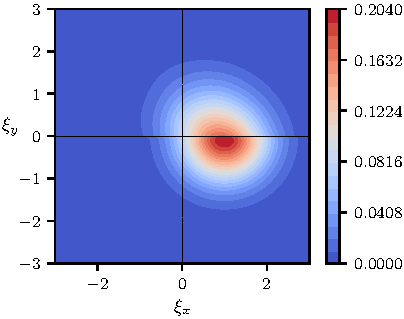
\includegraphics[width=\linewidth]{{{couette/kn0.1-boundary}}}
            \caption{Возле границы \(y=0.4990\)}
        \end{figure}
        \column{.55\textwidth}
        \begin{figure}
            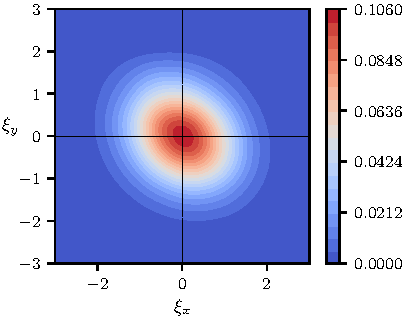
\includegraphics[width=\linewidth]{{{couette/kn0.1-center}}}
            \caption{Вблизи центра \(y=0.0082\)}
        \end{figure}
    \end{columns}
\end{frame}

\begin{frame}
    \frametitle{Функция распределения \(\Delta{v}=2\), срез \(\xi_z=0.1665\)}
    \vspace{-20pt} \[ Kn=1 \] \vspace{-20pt}
    \begin{columns}
        \column{.55\textwidth}
        \begin{figure}
            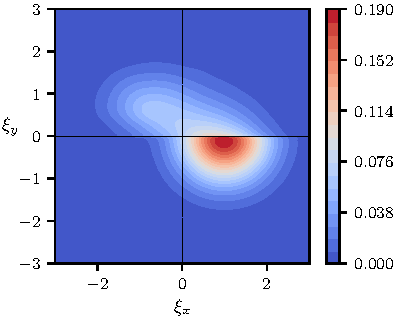
\includegraphics[width=\linewidth]{{{couette/kn1.0-boundary}}}
            \caption{Возле границы \(y=0.4929\)}
        \end{figure}
        \column{.55\textwidth}
        \begin{figure}
            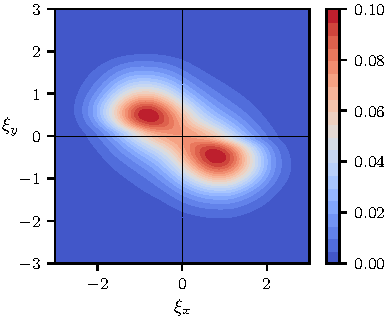
\includegraphics[width=\linewidth]{{{couette/kn1.0-center}}}
            \caption{Вблизи центра \(y=0.0083\)}
        \end{figure}
    \end{columns}
\end{frame}

\begin{frame}
    \frametitle{Функция распределения \(\Delta{v}=2\), срез \(\xi_z=0.1665\)}
    \vspace{-20pt} \[ Kn=10 \] \vspace{-20pt}
    \begin{columns}
        \column{.55\textwidth}
        \begin{figure}
            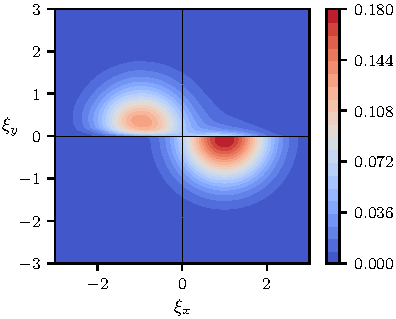
\includegraphics[width=\linewidth]{{{couette/kn10-boundary}}}
            \caption{Возле границы \(y=0.4917\)}
        \end{figure}
        \column{.55\textwidth}
        \begin{figure}
            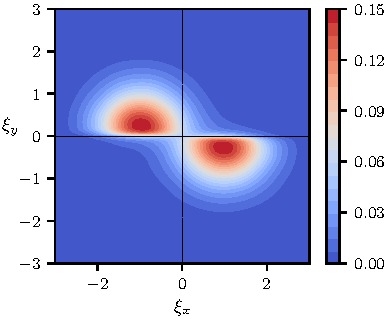
\includegraphics[width=\linewidth]{{{couette/kn10-center}}}
            \caption{Вблизи центра \(y=0.0083\)}
        \end{figure}
    \end{columns}
\end{frame}

\begin{frame}
    \frametitle{Логарифмические сингулярности}
    \begin{itemize}
        \item \Cite[2014]{Chen, Liu, Takata}
        \[ \pder[f]{x_i}n_i = \frac{C}{\Kn}\ln\frac{(x_i-x_{Bi})n_i}{\Kn} + \OO{1}. \]
        \item \Cite[2016]{Chen, Funagane, Liu, Takata}
        \[ \pder[f]{\xi_i}n_i = C\ln\xi_in_i + \OO{1}. \]
    \end{itemize}
    где \(x_{Bi}\) "--- координата граничной поверхности.
\end{frame}

\begin{frame}
    \frametitle{Профили сдвигового напряжения}
    \[ p_{xy} = -\Gamma_1(T_H)\der[v_H]{y}k + \OO{k^3} \]
    \centering
    \includegraphics[width=0.9\linewidth]{couette/Pxy}
\end{frame}

\begin{frame}
    \frametitle{Профили продольной скорости}
    \vspace{-5pt}
    \[ v = v_H - \frac{Y_0^--Y_0^+}{p_H}\left(T_H\der[v_H]{y}\right)_{y=\frac12}k + \OO{k^2} \]
    \vspace{-5pt}
    \centering
    \includegraphics[width=0.9\linewidth]{couette/vx}
\end{frame}

\begin{frame}
    \frametitle{Профили температуры}
    \vspace{-5pt}
    \[ T = T_H - \frac{\Theta_1^-+\Theta_1^+}{p_H}\left(T_H\der[T_H]{y}\right)_{y=\frac12}k + \OO{k^2} \]
    \vspace{-5pt}
    \centering
    \includegraphics[width=0.9\linewidth]{couette/tau}
\end{frame}

\begin{frame}
    \frametitle{Профили поперечного теплового потока}
    \[ q_y = -\frac54\Gamma_2(T_H)\der[T_H]{y}k + q_{yK2}k^2 + \OO{k^3} \]
    \centering
    \includegraphics[width=0.9\linewidth]{couette/qy}
\end{frame}

\begin{frame}
    \frametitle{Профили продольного теплового потока}
    \vspace{-10pt}
    \[ q_x = q_{xK1}k
        + \frac{T_H}{p_H}\left( \frac{\Gamma_3}2 \derdual[v_H]{y}
            + 4\Gamma_{10} \der[T_H]{y}\der[v]{y} \right)k^2
        + q_{xK2}k^2 + \OO{k^3} \]
    \vspace{-10pt}
    \centering
    \includegraphics[width=0.9\linewidth]{couette/qx}
\end{frame}

\begin{frame}
    \frametitle{Профили \(P_{xx}-P{yy}\)}
    \vspace{-15pt}
    \[ P_{xx}-P_{yy} = \left[ 2\Gamma_9 \left(\der[v_H]{y}\right)^2
        - \Gamma_3 \derdual[T_H]{y}
        - \Gamma_7\left(\der[T_H]{y}\right)^2 \right]\frac{k^2}{p_H} + \OO{k^3} \]
    \vspace{-15pt}
    \centering
    \includegraphics[width=0.9\linewidth]{couette/Pxx}
\end{frame}

\begin{frame}
    \frametitle{Профили \(P_{zz}-P{yy}\)}
    \footnotesize
    \vspace{-15pt}
    \[ P_{zz}-P_{yy} = \left[ 2(\Gamma_9-\Gamma_8) \left(\der[v_H]{y}\right)^2
        - \Gamma_3 \derdual[T_H]{y}
        - \Gamma_7\left(\der[T_H]{y}\right)^2 \right]\frac{k^2}{p_H} + \OO{k^3} \]
    \vspace{-15pt}
    \centering
    \includegraphics[width=0.9\linewidth]{couette/Pzz}
\end{frame}

\begin{frame}
    \frametitle{Транспортные коэффициенты для модели твёрдых сфер}
    \begin{alignat*}{2}
        \gamma_1 &= 1.270042427, \quad &\text{\Cite[1957]{Pekeris, Alterman}} \\
        \gamma_2 &= 1.922284065, \quad &\text{\Cite[1957]{Pekeris, Alterman}} \\
        \gamma_3 &= 1.947906335, \quad &\text{\Cite[1992]{Ohwada, Sone}} \\
        \gamma_7 &= 0.189200,    \quad &\text{\Cite[1996]{\footnotesize Sone, Aoki, Takata, Sugimoto, Bobylev}} \\
        \gamma_8 &= 1.495941968, \quad &\text{\Cite[2016]{Rogozin}} \\
        \gamma_9 &= 1.636073458, \quad &\text{\Cite[2016]{Rogozin}} \\
        \gamma_{10} &= 2.4497795.\quad &\text{\Cite[2016]{Rogozin}}
    \end{alignat*}
\end{frame}

\begin{frame}
    \frametitle{Зависимость сдвигового напряжения от \(\Kn\)}
    \vspace{-2pt}
    \centering\hspace{-1.5cm}
    \includegraphics[width=1.1\linewidth]{couette2/shear}
    \hspace{-1.5cm}
\end{frame}

\begin{frame}
    \frametitle{Зависимость продольной скорости от \(\Kn\)}
    \vspace{-2pt}
    \centering\hspace{-1.5cm}
    \includegraphics[width=1.1\linewidth]{couette2/flow}
    \hspace{-1.5cm}
\end{frame}

\begin{frame}
    \frametitle{Зависимость продольного теплового потока от \(\Kn\)}
    \vspace{-2pt}
    \centering\hspace{-1.5cm}
    \includegraphics[width=1.1\linewidth]{couette2/qflow}
    \hspace{-1.5cm}
\end{frame}

\begin{frame}
    \frametitle{Зависимость поперечного теплового потока от \(\Kn\)}
    \vspace{-2pt}
    \centering\hspace{-1.5cm}
    \includegraphics[width=1.1\linewidth]{couette2/qflowy}
    \hspace{-1.5cm}
\end{frame}

\begin{frame}
    \frametitle{Зависимость \(P_{zz}-P_{yy}\) от \(\Kn\)}
    \vspace{-2pt}
    \centering\hspace{-1.5cm}
    \includegraphics[width=1.1\linewidth]{couette2/pzz}
    \hspace{-1.5cm}
\end{frame}

\begin{frame}
    \frametitle{Заключение}
    \begin{enumerate}
        \item Удаётся детально разрешить плоские кинетические слои,
        но можно моделировать гиперзвуковые течения с большим перепадом температур.
        \item Вопрос сходимости, особенно влияния проекционного шаблона
        и отрицательных проекционных весов на её скорость.
        \item Нелинейная асимптотическая теория "--- хороший инструмент для верификации
        численных методов.
        \item Гидродинамическое описание газа может оказаться некорректным на масштабах существенно больше длины свободного пробега,
        если градиенты макроскопических величин в некоторых областях сравнимы с обратным числом Кнудсена.
    \end{enumerate}
\end{frame}

\end{document}
